
% !TEX TS-program = pdflatex
% !TEX encoding = UTF-8 Unicode

% This is a simple template for a LaTeX document using the "article" class.
% See "book", "report", "letter" for other types of document.

\documentclass[11pt]{article} % use larger type; default would be 10pt

\usepackage[utf8]{inputenc} % set input encoding (not needed with XeLaTeX)

%%% Examples of Article customizations
% These packages are optional, depending whether you want the features they provide.
% See the LaTeX Companion or other references for full information.

%%% PAGE DIMENSIONS
\usepackage{geometry} % to change the page dimensions
\geometry{a4paper} % or letterpaper (US) or a5paper or....
% \geometry{margin=2in} % for example, change the margins to 2 inches all round
% \geometry{landscape} % set up the page for landscape
%   read geometry.pdf for detailed page layout information

\usepackage{graphicx} % support the \includegraphics command and options

% \usepackage[parfill]{parskip} % Activate to begin paragraphs with an empty line rather than an indent

%%% PACKAGES
\usepackage{booktabs} % for much better looking tables
\usepackage{array} % for better arrays (eg matrices) in maths
\usepackage{paralist} % very flexible & customisable lists (eg. enumerate/itemize, etc.)
\usepackage{verbatim} % adds environment for commenting out blocks of text & for better verbatim
\usepackage{subfig} % make it possible to include more than one captioned figure/table in a single float
% These packages are all incorporated in the memoir class to one degree or another...

%%% HEADERS & FOOTERS
\usepackage{fancyhdr} % This should be set AFTER setting up the page geometry
\pagestyle{fancy} % options: empty , plain , fancy
\renewcommand{\headrulewidth}{0pt} % customise the layout...
\lhead{}\chead{}\rhead{}
\lfoot{}\cfoot{\thepage}\rfoot{}

%%% SECTION TITLE APPEARANCE
\usepackage{sectsty}
\allsectionsfont{\sffamily\mdseries\upshape} % (See the fntguide.pdf for font help)
% (This matches ConTeXt defaults)

%%% ToC (table of contents) APPEARANCE
\usepackage[nottoc,notlof,notlot]{tocbibind} % Put the bibliography in the ToC
\usepackage[titles,subfigure]{tocloft} % Alter the style of the Table of Contents
\renewcommand{\cftsecfont}{\rmfamily\mdseries\upshape}
\renewcommand{\cftsecpagefont}{\rmfamily\mdseries\upshape} % No bold!

\makeatletter
   \newcommand\figcaption{\def\@captype{figure}\caption}
   \newcommand\tabcaption{\def\@captype{table}\caption}
\makeatother
%%% END Article customizations

%%% The "real" document content comes below...

\title{CSE 509 Lecture 20}

\author{Prof. R. Sekar, Scribe:Arun Rathakrishnan}
%\date{} % Activate to display a given date or no date (if empty),
         % otherwise the current date is printed 

\begin{document}
\maketitle
\section {Blackbox Taint Tracking Technique}
Fine grained dynamic taint tracking requires source code instrumentation and 
policies setup at each function call. There is significant runtime overhead 
as a result, the approach is intrusive and requires a special complier to 
maintain, the tag bits and shadow stack. The alternative is to intercept the
HTTP requests as input to the webserver and consider requests from webserver
like sending a HTTP response or issuing a query to a database server as output.
\subsection {Comparison of Input and Output}
In this approach, the HTTP request is intercepted by plugins for Apache server,
which tracks a session ID to match a request message with another output message.
The data in the request is collected and represented as name-value pairs, which
is used by the rest of the system. Any output message from the webserver is matched
by the session ID and the system checks if the output and input messages have
similarity. This represents the taintedness of the message, which indicates the
amount of control, the user exerts on the program behaviour. We can do this
by checking if, the input has a common substring or subsequence with the output.
The latter approach is more robust.

\subsection {SQL/Command Injection}
An attacker usually injects SQL code, by introducing a new SQL statement with
a semicolon.
\begin {verbatim}
$cmd = "SELECT price FROM products WHERE name = ’" . $name . "’";
\end {verbatim}
The name is usually read from the HTTP request, which is typically passed from
a user input from a form. The user can input the below instead of a name and
can set prices in products table to $0$.
\begin {verbatim}
name = ’xyz’; UPDATE products SET price = 0 WHERE true
\end {verbatim}
This can be prevented by scanning the user input and looking for malicious
characters like ';'. But the identification is not that simple.
\subsection {Taint Tracking And Policies}
The system needs to determine,
\begin {itemize} \itemsep -2pt
\item Determine how much control is exerted by the user, through taint tracking.
\item If the contorl exerted is reasonable, by setting up policies.
\end {itemize}
\section{Syntax And Taint Aware Policy}
As shown above, the presence of ';' as a statement delimiter generally means that, the
tainted output message possibly contains an SQL injection. But if ';' occurs
within quotes or in any form other than as a statement delimiter, the message
is valid. Thus we can say that simple string matching can not enforce a strong
policy.\\
\begin {center}
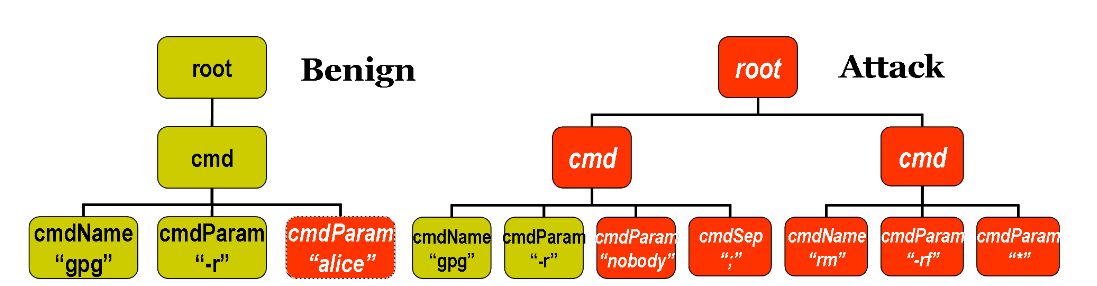
\includegraphics [width=350px,height=200px]{img/f1.png} \\
\caption {Syntatic Structure captures Command Injection [1]}
\end {center}
\subsection {Syntatic Structure}
An attack typically causes a change in syntatic structure of the query being
executed as shown above. In general, if the input spans more than one token,
and if the tainted tokens correspond to SQL or shell commands we can say that
an injection attack has been attempted. Thus knowledge of syntax and taintedness
helps detect attacks in general. An application and language independent approach
to this problem is undertaken in [1].
\subsection {Buffer Overflow}
In addition to injection attacks, taint tracking can detect memory errors like
buffer overflow. This can be done by checking if any code pointer (function
pointer or return address) is changed before calling or making a jump to another
instruction.  If the code pointer is tainted, it means that user input has been
written into the location, thus detecting buffer overflows and stack smashing
accurately.
\section {Static Analysis: Model Checking}
A model captures the behaviour of a system. A program can be represented as a
model. Model checking statically find errors in a program given a set of property
specifications. Property specifications can describe expected behaviour or deviations
from expected behaviour. From a security perspectve we are interested in two
types of properties rules of correctness or violations of correctness.
\subsection {Example: Root Privilege in FTP Server}
A FTP server process for an authenticated user needs root privileges for certain
actions like binding to a new port. The privlege must be acquired before the
bind operation and must be relinquished immediately after it.
\begin {verbatim}
    old_id = geteuid();
    setuid(0); \\Acquire root privilege
    bind();
    setuid(old_id);
\end {verbatim}	
\\ After acquiring root privilege the process should not perform any other system
call. For example, it should not call the system function.
\begin {verbatim}
    old_id = geteuid();
    setuid(0); \\Acquire root privilege
    system(input);
    setuid(old_id);
\end {verbatim}	
\subsection {Models and Properties}
Models can be represented Finite State Machine, Context Free Grammar, etc. Here
we consider only the FSM. Even though the model is finite, a small memory of
100 bytes can represent ${2^{800}}$ states. There is an explosion of statespace
and its important to keep the statespace small.\\

Properties can be classified into two,
\begin {itemize} \itemsep -2pt
\item Saftey: bad things never happen.
\item Liveness: good things eventually happen.
\end {itemize}
Liveness can not be modelled FSM. They can be represented by models like Buchi
automata.
\begin {center}
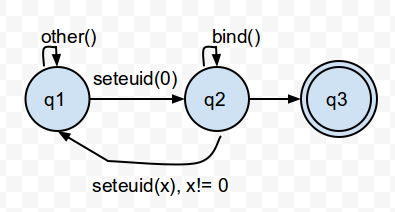
\includegraphics [width=260px,height=160px]{img/f2.png} \\
\caption {FSM For violation of root previlege}
\end {center}
%Pic: Bad automata.
The above FSM captures a bad property discussed in the above example, namely
misuse of root privilege by FTP Server process.

\subsection {Analysis}
Given a model $M$, and a property $P$, model checking involves finding if $M \cap
P$ has a path that leads to a bad state in $P$. Then the model is said to have an
error.
%Pic: Model

\begin {center}
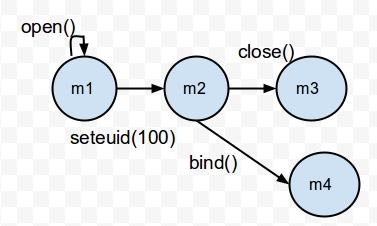
\includegraphics [width=260px,height=160px]{img/f3.png} \\
\caption {Model for FTP server process}
\end {center}

In model checking, the model $M$ for a program can be checked against a set of
properties to determine if the program does not violate some conditions encoded
by the properties.

\begin {center}
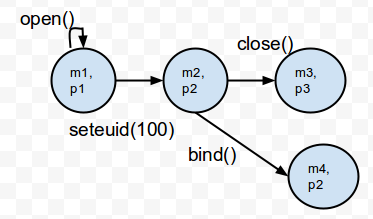
\includegraphics [width=300px,height=180px]{img/f4.png} \\
\caption {Model checking FTP Server}
\end {center}

\section {Reference}
R. Sekar, "An Efficient Black-box Technique for Defeating Web Application Attacks".   

\end{document}

